\documentclass[12pt, letterpaper]{article}

\usepackage{tikz}
\usepackage{pgfplots}
\pgfplotsset{width=7cm, compat=1.16}
\usepgfplotslibrary{statistics}
\usepackage{amsmath}

\title{Homework 2}
\author{Martin Mueller}
\date{Due: February $15^{th}$, 2019}

\begin{document}
\maketitle

\begin{center}
	\textbf{Chapter 1}
\end{center}

1. [The unit for all numbers below is miles.]

\qquad d) Below are the calculated values for the lower fourth, median, and upper fourth:
$$\text{Lower fourth}=12^{th}\text{ number in the set}=\boxed{31.4}$$
$$\text{Median}=23^{rd}\text{ number in the set}=\boxed{33.2}$$
$$\text{Upper fourth}=34^{th}\text{ number in the set}=\boxed{34.8}$$
\qquad e) Below is a box plot constructed with the values from above. A few extra values also used to draw the box plot are given as well:
$$\text{Fourth spread}=\text{Upper fourth}-\text{Lower fourth}=34.8-31.4=\boxed{3.4}$$
$$\text{Lower outlier bound}=\text{Lower fourth}-1.5\text{(Fourth spread)}=31.4-1.5(3.4)=\boxed{26.3}$$
$$\text{Lower extreme outlier bound}=\text{Lower fourth}-3\text{(Fourth spread)}=31.4-3(3.4)=\boxed{21.2}$$
$$\text{Upper outlier bound}=\text{Upper fourth}+1.5\text{(Fourth spread)}=34.8+1.5(3.4)=\boxed{39.9}$$
$$\text{Upper extreme outlier bound}=\text{Upper fourth}+3\text{(Fourth spread)}=34.8+3(3.4)=\boxed{45.0}$$
\begin{center}
	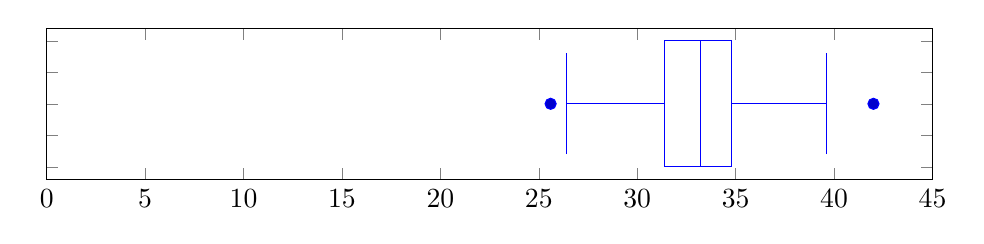
\begin{tikzpicture}
		\begin{axis}[
			xmin=0,
			xmax=45,
			x=0.25cm,
			y=2cm,
			yticklabels={,,}
		]
			\addplot+ [
				boxplot prepared={
					lower whisker=26.4,
					lower quartile=31.4,
					median=33.2,
					upper quartile=34.8,
					upper whisker=39.6,
				},
			]
			table [row sep=\\,y index=0] {
				data\\ 25.6\\ 42.0\\
			};
		\end{axis}
	\end{tikzpicture}
\end{center}

As you can see, there are two mild outliers in the data set: $25.6$ on the low end and $42.0$ on the high end.

\pagebreak

2. [The unit for all numbers below is minutes.]

\qquad d) Below are the calculated values for the lower fourth, median, and upper fourth:
$$\text{Lower fourth}=13^{th}\text{ number in the set}=\boxed{17.5}$$
$$\text{Median}=\frac{25^{th}\text{ number}+26^{th}\text{ number}}{2}=\frac{19.2+19.4}{2}=\boxed{19.3}$$
$$\text{Upper fourth}=38^{th}\text{ number in the set}=\boxed{20.6}$$
\qquad e) Below is a box plot constructed with the values from above. A few extra values also used to draw the box plot are given as well:
$$\text{Fourth spread}=\text{Upper fourth}-\text{Lower fourth}=20.6-17.5=\boxed{3.1}$$
$$\text{Lower outlier bound}=\text{Lower fourth}-1.5\text{(Fourth spread)}=17.5-1.5(3.1)=\boxed{12.9}$$
$$\text{Lower extreme outlier bound}=\text{Lower fourth}-3\text{(Fourth spread)}=17.5-3(3.1)=\boxed{8.2}$$
$$\text{Upper outlier bound}=\text{Upper fourth}+1.5\text{(Fourth spread)}=20.6+1.5(3.1)=\boxed{25.2}$$
$$\text{Upper extreme outlier bound}=\text{Upper fourth}+3\text{(Fourth spread)}=20.6+3(3.1)=\boxed{29.9}$$
\begin{center}
	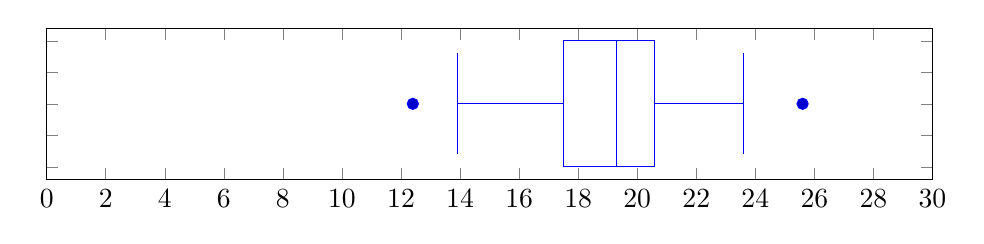
\begin{tikzpicture}
		\begin{axis}[
			xmin=0,
			xmax=30,
			x=0.375cm,
			y=2cm,
			yticklabels={,,}
		]
			\addplot+ [
				boxplot prepared={
					lower whisker=13.9,
					lower quartile=17.5,
					median=19.3,
					upper quartile=20.6,
					upper whisker=23.6,
				},
			]
			table [row sep=\\,y index=0] {
				data\\ 12.4\\ 25.6\\
			};
		\end{axis}
	\end{tikzpicture}
\end{center}

As you can see, there are two mild outliers in the data set: $12.4$ on the low end and $25.6$ on the high end.

\pagebreak

\begin{center}
	\textbf{Chapter 2}
\end{center}

1. Consider an experiment involving tossing a fair coin twice, and then rolling a fair once.

\qquad a) Listed below are all the possible outcomes of tossing a fair coin twice and rolling a fair die once; (Note: The outcomes of the coin or die landing on its side have been excluded):
\begin{center}
	\begin{align*}
		S = \{\quad &TT1, & &TH1, & &HT1, & &HH1, \quad\} \\
			   		&TT2, & &TH2, & &HT2, & &HH2,		  \\
			 	  	&TT3, & &TH3, & &HT3, & &HH3,		  \\
			   		&TT4, & &TH4, & &HT4, & &HH4,		  \\
			   		&TT5, & &TH5, & &HT5, & &HH5,		  \\
			   		&TT6, & &TH6, & &HT6, & &HH6
	\end{align*}
\end{center}

\qquad b) The only outcomes that are listed here are the ones where only one coin comes up heads and the number rolled on the die is a multiple of $2$:
\begin{center}
	\begin{align*}
		S = \{\quad &TH2,\quad HT2, \quad\} \\
			   		&TH4,\quad HT4,		  \\
			   		&TH6,\quad HT6
	\end{align*}
\end{center}

2. A sample of 3 batteries is selected from a manufacturing line, and each battery is classified as either defective or non-defective.  Let A, B and C denote the events that the first, second and third battery, respectively, are defective.

\qquad a) Listed below are all possible outcomes in the sample space for the above experiment:
$$S = \{\;A'B'C',\;A'B'C,\;A'BC',\;A'BC,\;AB'C',\;AB'C,\;ABC',\;ABC\;\}$$

\qquad b) Listed below are all possible outcomes in A:
$$S = \{\;AB'C',\;AB'C,\;ABC',\;ABC\;\}$$

\pagebreak

\qquad c) Listed below are all possible outcomes in $A \cup B$:
$$S = \{\;A'BC',\;A'BC,\;AB'C',\;AB'C,\;ABC',\;ABC\;\}$$

\qquad d) Listed below are all possible outcomes in $A \cap B$:
$$S = \{\;ABC',\;ABC\;\}$$

\qquad e) Listed below are all possible outcomes in $B \cup C$:
$$S = \{\;A'B'C,\;A'BC',\;A'BC,\;AB'C,\;ABC',\;ABC\;\}$$

3. A survey of 1000 students at a large university shows that 750 students own stereos, 450 own cars, and 350 own cars and stereos. Let event A mean that a student owns a stereo, and let event B mean that a student owns a car. If a student at the university is selected at random, find the probability that...

\qquad a) ...the student owns either a car or a stereo.
\begin{center}
	\begin{align*}
		P(A) &= \frac{750 \text{ students}}{1000 \text{ students}} = 0.75 \\
		P(B) &= \frac{450 \text{ students}}{1000 \text{ students}} = 0.45 \\
		P(A \cap B) &= \frac{350 \text{ students}}{1000 \text{ students}} = 0.35 \\
		\\
		\text{Addition Rule: } A \cup B &= P(A) + P(B) - P(A \cap B) \\
		&= 0.75 + 0.45 - 0.35 \\
		&= \boxed{0.85}
	\end{align*}
	However, that is if "or" is taken here to be inclusive. If it is exclusive in this context, then we would need to subtract an additional $P(A \cap B)$:
	$$0.85-0.35=\boxed{0.50}$$
\end{center}

\qquad b) ...the student owns neither a car nor a stereo.
\begin{center}
	Since this is the compliment of the event above (in the inclusive case), I can simply use the fact that the compliment of a given event is simply $1$ minus the probability of that event. I will call the event above event C.
	$$P(C') = 1 - P(C) = 1 - 0.85 = \boxed{0.15}$$
\end{center}

\pagebreak

\qquad c) ...the student owns only a stereo.
\begin{center}
	I will use some of the results obtained in a) to get an answer here:
	\begin{align*}
		P(A) &= 0.75 \\
		P(A \cap B) &= 0.35 \\
		\\
		P(\text{the student only owns a stereo}) &= P(\text{students owns a stereo}) \\
		&\quad- P(\text{student also owns a car}) \\
		&= P(A) - P(A \cap B) \\
		&= 0.75 - 0.35 \\
		&= \boxed{0.40}
	\end{align*}
\end{center}

4. The probability that an integrated circuit chip will have defective etching is  0.12, the probability it will have a crack defect is 0.29, and the probability that it has both defects is 0.07. Let A be the event where the chip has defective etching, and let B be the event where the chip has a crack defect.  Find the probability that a newly manufactured chip will...

\qquad a) ...have either an etching or a crack defect.
\begin{center}
	Just like in 3a, we can use the addition rule and substitute in the values of the three given probabilities:
	\begin{align*}
		P(A) &= 0.12 \\
		P(B) &= 0.29 \\
		P(A \cap B) &= 0.07 \\
		\\
		\text{Addition Rule: } A \cup B &= P(A) + P(B) - P(A \cap B) \\
		&= 0.12 + 0.29 - 0.07 \\
		&= \boxed{0.34}
	\end{align*}
	However, that is if "or" is taken here to be inclusive. If it is exclusive in this context, then we would need to subtract an additional $P(A \cap B)$:
	$$0.34 - 0.07 = \boxed{0.27}$$
\end{center}

\pagebreak

\qquad b) ...have neither defect.
\begin{center}
	Since this is the compliment of the event above (in the inclusive case), I can simply use the fact that the compliment of a given event is simply $1$ minus the probability of that event. I will call the event above event C.
	$$P(C') = 1 - P(C) = 1 - 0.34 = \boxed{0.66}$$
\end{center}

\qquad c) ...have an etching defect only.
\begin{center}
	I will use some of the results used in a) to get an answer here:
	\begin{align*}
		P(A) &= 0.12 \\
		P(A \cap B) &= 0.07 \\
		\\
		P(\text{the chip on has an etching defect}) &= P(\text{chip has an etching defect}) \\
		&\quad- P(\text{the chip also has a crack defect}) \\
		&= P(A) - P(A \cap B) \\
		&= 0.12 - 0.07 \\
		&= \boxed{0.05}
	\end{align*}
\end{center}
\end{document}